\section{ \textbf{State of the Art: GPU Research} }
\label{sec:SOTAGPU}

In this section, we will be considering recent advances in Monte Carlo research on GPU architectures.
%
We will first survey different approaches for utilizing the GPU. 
%
We will then survey Monte Carlo transport from the medical transport perspective in order compare approaches from the different communities.
%
Then we will survey uses of ray tracing within a Monte Carlo transport application.
%
Finally, we will survey new algorithm choices through event based Monte Carlo transport.
%

%
\subsection{\textbf{ Comparing CPU and GPU Architectures} }

``A simple way to understand the difference between a CPU and GPU is to compare how they process tasks. A CPU consists of a few cores optimized for sequential serial processing while a GPU has a massively parallel architecture consisting of thousands of smaller, more efficient cores designed for handling multiple tasks simultaneously." -- NVidia website~\cite{CPUvGPUnvidia}

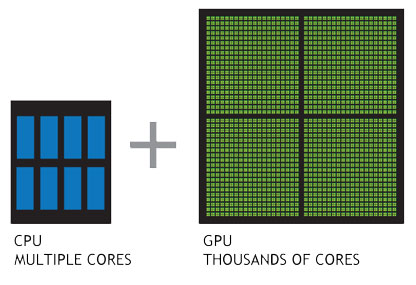
\includegraphics[width=0.4\textwidth]{cpu-and-gpu.jpg}~\cite{CPUvGPUnvidia}

A CPU has been developed to optimize the performance of a single task. 
%
In order to accomplish this CPUs have been latency optimized, meaning that the time to complete one task, including gathering the necessary memory, has been reduced in any way possible.
%
GPUs, on the other hand have been throughput optimized in order to complete as many tasks as possible in a given amount of time.
%
This means that the time for a GPU to complete a single task is most likely significantly longer than for a CPU, but, in a fixed amount of time the GPU will be able to accomplish many more tasks.
%
So given a large enough number of tasks that can be carried out in parallel, the GPU can likely execute faster.


